\documentclass[journal,onecolumn]{IEEEtran}

% * CITATION PACKAGES *
\usepackage{cite}

% * GRAPHICS RELATED PACKAGES *
\usepackage{graphicx}
\graphicspath{{./}{../}}
\DeclareGraphicsExtensions{.pdf,.jpeg,.jpg,.png}

% * MATH PACKAGES *
\usepackage{amsmath}
\usepackage{amssymb}
\usepackage{amsfonts}

% * ALIGNMENT PACKAGES *
\usepackage{array}

% * PDF, URL AND HYPERLINK PACKAGES *
\usepackage{url}
\usepackage{booktabs}
\usepackage{microtype}
\usepackage[hidelinks]{hyperref}
\usepackage{float}

% Correct bad hyphenation here
\hyphenation{op-tical net-works semi-conduc-tor}

\begin{document}

% Paper title
\title{Semantic-Aware Integrated Sensing and Communication (ISAC) Networks with Power-Domain NOMA and 3D Elevation-Dependent Path Loss}

% Author names and affiliations
\author{
Nikhil~Gadige,
Anuj~Saha,
Divyanshu~Ghosh,
and Mohli~Thapa%
\thanks{N. Gadige, A. Saha, D. Ghosh, and M. Thapa are with the Department of Computer Science and Engineering, Indian Institute of Information Technology Vadodara, under the Summer Research Program 2026.}%
\thanks{E-mails: 202351037@iiitvadodara.ac.in, 202351010@iiitvadodara.ac.in, 202351036@iiitvadodara.ac.in, 202351084@iiitvadodara.ac.in.}
}

% Make the title area
\maketitle

\begin{abstract}
Integrated Sensing and Communication (ISAC) has emerged as a key technology for 6G wireless systems to share spectrum and hardware resources efficiently. However, resource scarcity and security vulnerability in Air-to-Ground (A2G) networks pose critical implementation challenges. In this report, we present the design and system model of a Semantic-Aware ISAC Network assisted by an aerial Reconfigurable Intelligent Surface (RIS) mounted on an Unmanned Aerial Vehicle (UAV) ($R$). To optimize spectral efficiency, we employ Power-Domain Non-Orthogonal Multiple Access (PD-NOMA) to serve a near user (Target $T$, which is the updated form of the vehicle node) and a distant mobile user ($U$) simultaneously. Crucially, all communications and sensing nodes operate under semantic-aware metrics, shifting the focus from error-free bit transmission to the preservation of meaning. To capture realistic aerial propagation, we integrate a 3D elevation-dependent path loss model that dynamically adjusts the Line-of-Sight (LoS) probability and Rician $K$-factor. Additionally, the system is subjected to directional jamming from a UAV Jammer ($J$), which also performs monostatic radar sensing. Eavesdropping nodes ($E_1, E_2, E_3$) are distributed to wiretap the downlink transmissions. We formulate the detailed mathematical models and signal flows for the entire network, providing a rigorous foundation for subsequent optimization and reinforcement learning studies.
\end{abstract}

\begin{IEEEkeywords}
Integrated Sensing and Communication (ISAC), Semantic Communications, Power-Domain NOMA, Reconfigurable Intelligent Surface (RIS), Air-to-Ground (A2G) Path Loss, Successive Interference Cancellation (SIC).
\end{IEEEkeywords}

\IEEEpeerreviewmaketitle

\section{Introduction}
Future 6G networks are envisioned to go beyond traditional communication by integrating radar sensing and semantic intelligence into a unified architecture. Integrated Sensing and Communication (ISAC) allows wireless nodes to simultaneously transmit information and sense environment parameters (e.g., target localization and tracking) using the same frequency bands and hardware.

To overcome severe blockages and path loss in urban environments, Reconfigurable Intelligent Surfaces (RIS) mounted on Unmanned Aerial Vehicles (UAVs) ($R$) can be deployed as passive aerial reflectors. By adjusting the phase shifts of the RIS elements, a virtual Line-of-Sight (LoS) link can be established between a terrestrial Base Station (BS) $B$ and ground users, dramatically increasing signal coverage and physical layer security.

In parallel, semantic communications represent a paradigm shift from Shannon's classical information theory, which focuses solely on the accurate transmission of bit sequences. Rather than guaranteeing bit-level fidelity, a semantic-aware transmitter extracts the task-relevant meaning of a message through a learned semantic encoder and conveys only a compact set of semantic symbols that are sufficient for the intended receiver to reconstruct that meaning. This approach drastically reduces the required channel symbols and increases resilience against severe fading and interference, while simultaneously offering an inherent security advantage: an intercepted semantic symbol stream is largely uninterpretable to any node that does not possess the same semantic encoder-decoder pair, since meaning recovery -- unlike bit recovery -- depends on shared semantic knowledge rather than on the raw symbols themselves.

This report outlines the implementation details and mathematical models completed during Week 9. We design a semantic-aware ISAC network incorporating:
\begin{enumerate}
    \item \textbf{Elevation-Dependent Path Loss}: Incorporating 3D elevation angle $\theta_{ij}$, sigmoidal LoS probability $P_{\text{LoS}}(\theta_{ij})$, and elevation-dependent Rician fading.
    \item \textbf{Power-Domain NOMA (PD-NOMA)}: Serving a near Target user ($T$) and a distant Mobile User ($U$) over a superposed downlink signal, using semantic-aware Successive Interference Cancellation (SIC), in which the near user first reconstructs the far user's semantic information and removes its contribution before decoding its own semantic symbols.
    \item \textbf{Semantic Performance Metrics}: Characterizing semantic similarity, semantic rate, and semantic distortion for downlink, uplink, V2X, and eavesdropper channels -- each governed by the semantic compression ratio between semantic concepts and transmitted channel symbols -- as well as semantic sensing accuracy at the radar receiver.
\end{enumerate}


\begin{figure}[H]
    \centering
    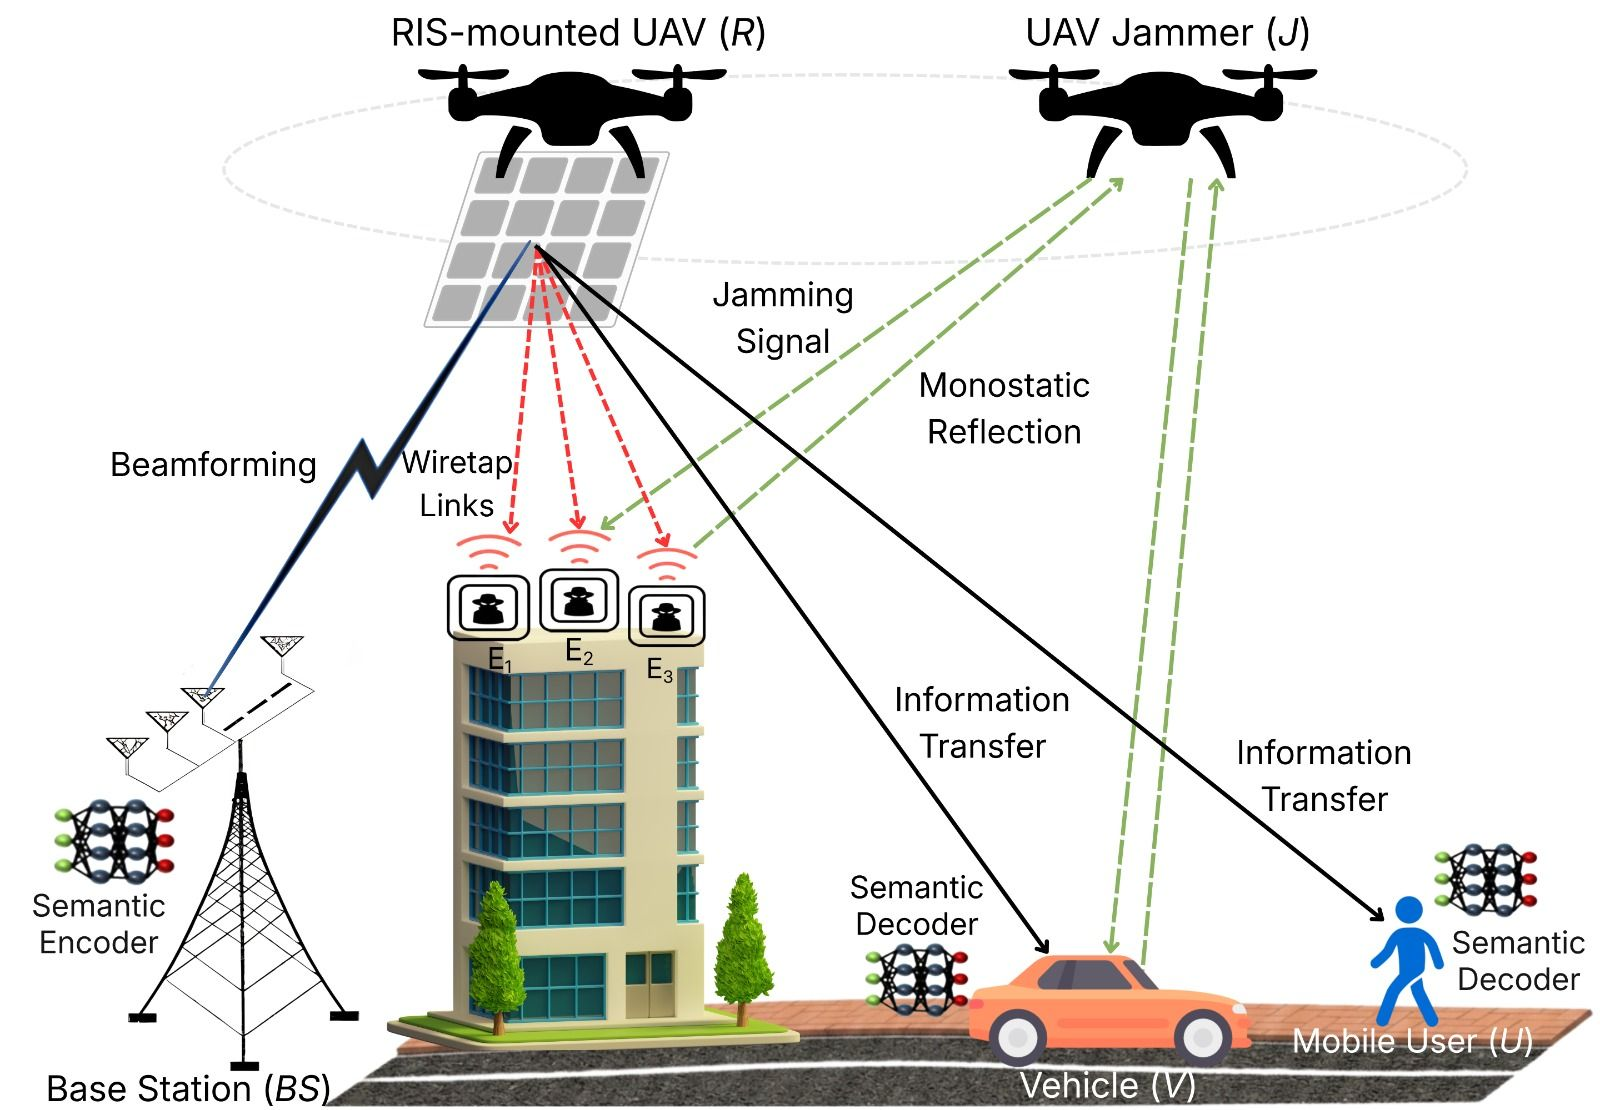
\includegraphics[width=\textwidth]{system-model.jpeg}
    \caption{System model of the proposed semantic-aware RIS-assisted UAV ISAC network. The Base Station (BS) communicates with the Target ($T$) and Mobile User ($U$) through an RIS-mounted UAV ($R$) using beamforming and PD-NOMA. A UAV Jammer ($J$) transmits jamming signals while performing monostatic sensing, whereas multiple eavesdroppers ($E_1$, $E_2$, and $E_3$) attempt to intercept the downlink transmissions. Semantic encoders and decoders are employed at the communicating nodes.}
    \label{fig:system_model}
\end{figure}

\section{System Architecture and Node Descriptions}
We consider an aerial-terrestrial co-existing network operating in a bounded 3D space. The system consists of the following key nodes:
\begin{itemize}
    \item \textbf{Base Station ($B$)}: Located at $\mathbf{p}_B = [x_B, y_B, z_B]^T$. It acts as a semantic-aware transmitter sending superposed downlink signals to paired users.
    \item \textbf{RIS-mounted UAV ($R$)}: An aerial platform hovering at $\mathbf{p}_R = [x_R, y_R, z_R]^T$, equipped with $N_R$ passive reflecting elements to establish cascaded communication paths.
    \item \textbf{UAV Jammer ($J$)}: An adversarial aerial node located at $\mathbf{p}_J = [x_J, y_J, z_J]^T$. It transmits directional jamming signals to degrade ground user rates while performing monostatic radar sensing reflections off the RIS $R$.
    \item \textbf{Target ($T$)}: A near user and active communicator (representing the updated form of the vehicle) located at $\mathbf{p}_T = [x_T, y_T, z_T]^T$. In the downlink, it decodes the NOMA signal using semantic-aware SIC. In the uplink, it transmits semantic messages to the Base Station $B$ (via the RIS $R$) and directly to the Mobile User $U$ via V2X.
    \item \textbf{Mobile User ($U$)}: A distant user located at $\mathbf{p}_U = [x_U, y_U, z_U]^T$, decoding the downlink far-user signal directly.
    \item \textbf{Eavesdroppers ($E_1, E_2, E_3$)}: Ground nodes located at positions $\mathbf{p}_{E_i}$, trying to intercept the downlink semantic transmissions.
\end{itemize}

\section{Mathematical Formulations}

Before detailing the individual link models, we first outline the end-to-end semantic communication pipeline that underlies every transmission in the network, from the Base Station downlink to the Target's uplink and V2X links. A semantic message originating at a \emph{semantic source} (e.g., a sentence, a sensor reading, or a control instruction) is first mapped by a \emph{semantic encoder}, implemented as a joint source-channel coding (JSCC) neural network, into a sequence of $M$ semantic concepts. These concepts are subsequently represented by $K$ transmitted channel symbols, where $K$ is generally much smaller than the number of bits required for a conventional, meaning-agnostic bit-level representation of the same message. The resulting semantic symbol stream is transmitted over the elevation-dependent wireless channel described in Section III-A, which introduces path loss, small-scale fading, jamming interference, and, where applicable, eavesdropping. At the legitimate receiver, a matched \emph{semantic decoder} maps the received (and possibly noisy) symbols back into an estimate of the original meaning. Formally, this pipeline can be summarized as
\[
\begin{aligned}
\text{Semantic Source}
&\rightarrow \text{Semantic Encoder (JSCC)}
\rightarrow \text{Semantic Symbols} \\
&\rightarrow \text{Wireless Channel}
\rightarrow \text{Semantic Decoder}
\rightarrow \text{Recovered Meaning}
\end{aligned}
\]
The ratio $M/K$, referred to as the \emph{semantic compression ratio}, governs the trade-off between transmission efficiency and semantic fidelity: a larger $M/K$ conveys more semantic concepts per transmitted symbol (higher efficiency) but places greater reconstruction burden on the semantic decoder under a given channel quality, generally increasing susceptibility to semantic distortion; a smaller $M/K$ trades efficiency for robustness. This compression ratio directly scales the semantic rate expression introduced in Section III-C and is treated identically across all downlink, uplink, V2X, and eavesdropper links considered in this report.

To formulate the system metrics, every received SINR that feeds a semantic decoder in this report (Sections III-B, III-D, and III-F) is represented by the symbol $\gamma$, which corresponds directly to the conventional physical link-budget SINR (transmit power scaled by channel gain, divided by jamming interference plus noise). Formally, for any link, the signal-to-interference-plus-noise ratio is:
\begin{equation}
    \gamma = \Gamma,
\end{equation}
where $\Gamma$ is the power-domain signal-to-interference-plus-noise ratio computed from transmit power, channel gain, jamming power, and $\sigma^2$ in the usual manner. This definition is applied consistently to every SINR expression in the remainder of the report, while the efficiency-reliability trade-off from compression is captured through the semantic rate conversion factor $M/K$ in Section III-C.

\subsection{Elevation-Dependent Air-to-Ground Path Loss and Channel Model}
For any propagation link $ij$ between a transmitter $i$ at position $\mathbf{p}_i = [x_i, y_i, z_i]^T$ and a receiver $j$ at $\mathbf{p}_j = [x_j, y_j, z_j]^T$ (with $ij \in \{BR, RT\}$ denoting the links from BS $B$ to RIS $R$ and RIS $R$ to Target $T$, respectively), the 3D Euclidean distance is:
\begin{equation}
    d_{ij} = \|\mathbf{p}_i - \mathbf{p}_j\|_2 = \sqrt{(x_i - x_j)^2 + (y_i - y_j)^2 + (z_i - z_j)^2}.
\end{equation}

The 2D horizontal distance is $d_{\text{2D}, ij} = \sqrt{(x_i - x_j)^2 + (y_i - y_j)^2}$. The vertical elevation difference is $\Delta z_{ij} = |z_i - z_j|$. The 3D elevation angle $\theta_{ij}$ (in degrees) is given by:
\begin{equation}
    \theta_{ij} = \arcsin\left( \frac{\Delta z_{ij}}{d_{ij}} \right) \cdot \frac{180}{\pi} = \arctan\left( \frac{\Delta z_{ij}}{d_{\text{2D}, ij}} \right) \cdot \frac{180}{\pi}.
\end{equation}

Due to the variations in building heights, blockages, and terrain, the probability of establishing a Line-of-Sight (LoS) link is modeled as a sigmoidal function of the elevation angle $\theta_{ij}$:
\begin{equation}
    P_{\text{LoS}}(\theta_{ij}) = \frac{1}{1 + a \cdot \exp\left( -b (\theta_{ij} - a) \right)},
\end{equation}
where $a$ and $b$ are calibration constants representing the urban environment (e.g., $a = 9.61, b = 0.16$ for typical urban environments). The Non-Line-of-Sight (NLoS) probability is $P_{\text{NLoS}}(\theta_{ij}) = 1 - P_{\text{LoS}}(\theta_{ij})$.

The path losses for the LoS and NLoS states, incorporating excessive attenuation, are modeled as:
\begin{equation}
    \text{PL}_{\text{LoS}}(d_{ij}) = 20\log_{10}\left( \frac{4\pi d_{ij} f_c}{c} \right) + \eta_{\text{LoS}},
\end{equation}
\begin{equation}
    \text{PL}_{\text{NLoS}}(d_{ij}) = 20\log_{10}\left( \frac{4\pi d_{ij} f_c}{c} \right) + \eta_{\text{NLoS}},
\end{equation}
where $f_c$ is the carrier frequency, $c$ is the speed of light, and $\eta_{\text{LoS}}$, $\eta_{\text{NLoS}}$ represent the excessive path loss factors in dB for LoS and NLoS links, respectively. The mean path loss in dB is:
\begin{equation}
    \overline{\text{PL}}(d_{ij}, \theta_{ij}) = P_{\text{LoS}}(\theta_{ij}) \cdot \text{PL}_{\text{LoS}}(d_{ij}) + \left(1 - P_{\text{LoS}}(\theta_{ij})\right) \cdot \text{PL}_{\text{NLoS}}(d_{ij}).
\end{equation}
Converting this to linear gain yields:
\begin{equation}
    \text{PL}_{\text{linear}}(d_{ij}, \theta_{ij}) = 10^{-\overline{\text{PL}}(d_{ij}, \theta_{ij}) / 10}.
\end{equation}

The small-scale fading envelope power gain is represented by $h$ throughout the paper (replacing $f$). For Rayleigh fading, the fading power gain is exponentially distributed with unit mean, i.e., $h \sim \text{Exp}(1)$. For Rician fading, we model the fading power gain as:
\begin{equation}
    h = |g_{\text{fade}}|^2, \quad g_{\text{fade}} = \sqrt{\frac{K}{K+1}} \bar{g}_{\text{fade}} + \sqrt{\frac{1}{K+1}} \tilde{g}_{\text{fade}},
\end{equation}
where $\bar{g}_{\text{fade}}$ is the deterministic LoS component, $\tilde{g}_{\text{fade}} \sim \mathcal{CN}(0, 1)$ is the scattered NLoS component, and $K$ is the Rician $K$-factor. In our model, $K$ scales with the elevation angle:
\begin{equation}
    K_{\text{dB}}(\theta_{ij}) = K_0 + \alpha_K \theta_{ij}, \quad K(\theta_{ij}) = 10^{K_{\text{dB}}(\theta_{ij}) / 10},
\end{equation}
where $K_0 = 3.0$ dB and $\alpha_K = 0.15$ dB/degree. The final channel power gain $g_{ij}$ is represented as:
\begin{equation}
    g_{ij} = \text{PL}_{\text{linear}}(d_{ij}, \theta_{ij}) \cdot h_{ij},
\end{equation}
where $h_{ij}$ represents the small-scale fading gain of link $ij$.

\subsection{Power-Domain NOMA and Semantic-Aware Successive Interference Cancellation}
In the downlink phase, the Base Station $B$ transmits a superposed signal to serve both the near user (Target $T$) and the far user (Mobile User $U$) using the same time-frequency resource. Under semantic communications, the signals $s_N$ and $s_F$ represent the semantic symbol sequences generated by deep learning joint source-channel coding (JSCC) encoders for the Target $T$ and Mobile User $U$, respectively -- that is, each of $s_N$ and $s_F$ already embodies the compressed semantic representation of its respective source message, following the pipeline introduced at the start of Section III, rather than a conventional bit-level codeword:
\begin{equation}
    s = \sqrt{a_N P_B} s_N + \sqrt{a_F P_B} s_F,
\end{equation}
where $P_B$ is the Base Station transmit power, and $a_N, a_F$ are the power allocation factors satisfying:
\begin{equation}
    a_N + a_F = 1, \quad a_F > a_N \ge 0.
\end{equation}

The signals propagate through the reflected cascaded link via the RIS $R$. The cascaded channel gain between the Base Station at position $\mathbf{p}_B$ and a destination user $k \in \{T, U\}$ at position $\mathbf{p}_k$ through the RIS $R$ at $\mathbf{p}_R$ is computed as:
\begin{equation}
    g_{\text{cascaded}, k} = g_{B, R} \cdot g_{R, k} \cdot N_R^2, \quad k \in \{T, U\},
\end{equation}
where $g_{B, R} = \text{PL}_{\text{linear}}(d_{B, R}, \theta_{B, R}) \cdot h_B$ (with $h_B$ representing small-scale fading on the BS-RIS link) and $g_{R, k} = \text{PL}_{\text{linear}}(d_{R, k}, \theta_{R, k}) \cdot h_R$ (with $h_R$ representing small-scale fading on the RIS-destination link) are the individual elevation-dependent channel gains, and $N_R$ is the number of RIS reflecting elements. The total effective channel gain for user $k \in \{T, U\}$ is:
\begin{equation}
    g_k = g_{\text{cascaded, } k}.
\end{equation}

For decoding, the users are ordered based on their effective channel gains. If $g_T < g_U$ due to shadowing or user mobility, the roles are swapped dynamically. Under normal conditions:
\begin{equation}
    g_T \ge g_U.
\end{equation}

The UAV Jammer $J$ emits artificial noise with power $P_J$, resulting in received jamming interference power at receiver $k \in \{T, U\}$:
\begin{equation}
    P_{J, k} = P_J \cdot g_{J, k},
\end{equation}
where $g_{J, k}$ is the elevation-dependent channel gain from the Jammer $J$ to receiver $k$. Note that for the Target $T$, the jamming interference is specifically denoted as $P_{J, T}$ (replacing the symbol $I_{\text{Jam}, \text{Veh}}$).

\subsubsection{Distant (Far) User Semantic Decoding}
The SINR at the Far User is:
\begin{equation}
    \gamma_F = \frac{a_F P_B g_U}{a_N P_B g_U + P_{J, U} + \sigma^2},
\end{equation}
where $P_{J, U} = P_J g_{J, U}$ is the jamming power received at Mobile User $U$, and $\sigma^2$ is the background thermal noise power. This SINR is passed directly through the semantic decoder's operating characteristic: the Mobile User evaluates the recovered meaning using its semantic similarity score $S_U(\gamma_F)$ and semantic rate $R_{\text{sem}, U}$ as detailed in Section III-C, rather than a conventional bit-error-rate criterion.

\subsubsection{Near User Semantic-Aware SIC Decoding}
The received SINR at the Target $T$ for decoding its own signal $s_N$ simplifies to:
\begin{equation}
    \gamma_N = \frac{a_N P_B g_T}{P_{J, T} + \sigma^2},
\end{equation}
where the denominator contains only the received Jammer interference $P_{J, T}$ and the background noise variance $\sigma^2$. Note that, since cancellation is performed on the semantic representation rather than on individual bits, any residual imperfection in reconstructing $\hat{s}_F$ manifests as semantic distortion rather than a conventional bit error, and is implicitly captured through the semantic similarity function of Section III-C. Under semantic communications, $\gamma_N$ is directly used to evaluate the semantic similarity score $S_T(\gamma_N)$ and the resulting semantic rate $R_{\text{sem}, T}$ as detailed in Section III-C.

\subsection{Semantic Communication Metrics}
For a semantic link, the receiver evaluates the performance using semantic-specific variables rather than bit error rates. The three metrics below -- semantic similarity, semantic rate, and semantic distortion -- are evaluated identically for every link in the network (downlink near- and far-user links, uplink V2I, V2X, and eavesdropper links) by substituting the corresponding link SINR $\gamma$, so that a single consistent semantic performance model applies throughout the report.

\subsubsection{Semantic Similarity Score $S(\gamma)$}
The similarity between the original sentence's semantic features and the reconstructed features at the receiver is obtained directly from a trained DeepSC model (Xie \emph{et al.}, \emph{Deep Learning Enabled Semantic Communication Systems}, IEEE TSP 2021), rather than from a hand-fitted closed-form curve. DeepSC realizes the semantic encoder/decoder pipeline of Section III as a Transformer-based semantic encoder, a dense channel encoder that maps semantic features to power-normalized channel symbols, an AWGN physical channel, a dense channel decoder, and a Transformer-based semantic decoder that reconstructs the sentence. The model is trained end-to-end with a token-level cross-entropy reconstruction loss while the transmit SINR is sampled uniformly at random per batch, so that a single trained network is evaluated consistently across the operating SINR range.

Once trained, the model is evaluated offline over a grid of fixed SINR values $\gamma_{\text{dB}}$; at each point the reconstructed sentence is decoded and compared against the original by cosine similarity of the semantic encoder's sentence embeddings (used here in place of an external BERT sentence-similarity model), averaged over the validation corpus and multiple channel noise realizations. This produces an empirical table $S(\gamma_{\text{dB}})$, which is linearly interpolated at simulation time (flat outside the trained range) to evaluate $S(\gamma)$ for any link SINR in the network:
\begin{equation}
    S(\gamma) = \operatorname{interp}\big(\gamma_{\text{dB}},\; \{(\gamma_{\text{dB}}^{(i)}, S^{(i)})\}_{i=1}^{N}\big), \qquad \gamma_{\text{dB}} = 10\log_{10}(\gamma),
\end{equation}
where $\{(\gamma_{\text{dB}}^{(i)}, S^{(i)})\}$ is the SINR-vs-similarity table produced by the trained DeepSC model. $S(\gamma) \in (0,1)$ saturates toward the model's achievable ceiling as the link SINR grows large, reflecting near-perfect meaning recovery under favorable channel conditions, and decays toward the model's near-total-failure floor as $\gamma$ degrades below the trained operating range, reflecting the collapse of semantic fidelity when the channel is too noisy for the decoder to recover the transmitted concepts. (Training, evaluation, and lookup-table generation are implemented in \texttt{train\_deepsc.py}; the interpolation used at simulation time is implemented in \texttt{deepsc\_lookup.py}.)

\subsubsection{Semantic Rate $R_{\text{sem}}$}
The semantic transmission rate, representing the number of semantic units transmitted per second, is defined as:
\begin{equation}
    R_{\text{sem}} = B \cdot \left( \frac{M}{K} \right) \cdot S(\gamma) \cdot \log_2(1 + \gamma) \quad (\text{suts/sec}),
\end{equation}
where $B$ is the link bandwidth, $M$ is the number of semantic concepts in a semantic unit, $K$ is the number of transmitted channel symbols, and $M/K$ represents the semantic compression ratio introduced at the beginning of Section III. This expression couples three distinct effects: the classical Shannon-type term $\log_2(1+\gamma)$, which bounds the raw information-carrying capacity of the channel at the semantic-effective SINR $\gamma$ defined in Section III-B; the semantic similarity factor $S(\gamma)$, which discounts that capacity by the fraction of transmitted symbols that are actually decoded into correct meaning; and the explicit compression ratio $M/K$, which converts the resulting channel-symbol rate into a rate of \emph{semantic units} per second. Note that $M/K$ therefore enters $R_{\text{sem}}$ twice, in two distinct roles: implicitly, through the $K/M$ dilution already embedded in $\gamma$ (which lowers both $\log_2(1+\gamma)$ and $S(\gamma)$ as compression increases), and explicitly, as the units-conversion multiplier $M/K$ in front. This combination produces the trade-off anticipated in Section III: increasing $M/K$ raises $R_{\text{sem}}$ through the explicit multiplier, but simultaneously lowers the semantic-effective SINR $\gamma$ and hence $S(\gamma)$ and $\log_2(1+\gamma)$ through the implicit $K/M$ dilution; the semantic rate is therefore maximized at an intermediate compression ratio rather than growing without bound as compression is increased, consistent with the qualitative discussion given earlier in this section.

\subsubsection{Semantic Distortion $D_{\text{sem}}$}
The average loss of semantic meaning due to channel impairments is quantified as:
\begin{equation}
    D_{\text{sem}} = 1 - S(\gamma).
\end{equation}
Since $S(\gamma)$ already reflects the joint effect of channel quality and compression aggressiveness through the semantic decoder's operating characteristic, $D_{\text{sem}}$ directly captures the residual meaning that is lost at the receiver, whether due to weak $\gamma$, high jamming interference, or an overly aggressive semantic compression ratio $M/K$ chosen at the encoder.

\subsection{Uplink Semantic Communication}
The Target $T$ also acts as an active terrestrial transmitter, encoding its uplink messages through the same semantic encoder pipeline described at the start of Section III before transmission.
\begin{itemize}
    \item \textbf{Uplink V2I (Target to BS via RIS R)}:
    The Target transmits its semantic signal with power $P_T$. The cascaded channel gain from the Target to the BS $B$ via the RIS $R$ is $g_{T, R, B}$, and $P_{J, B} = P_J g_{J, B}$ is the received jamming interference at the BS $B$ from Jammer $J$. The SINR $\gamma_{\text{uplink}}$ at the BS $B$ is:
    \begin{equation}
        \gamma_{\text{uplink}} = \frac{P_T g_{T, R, B}}{P_{J, B} + \sigma^2}.
    \end{equation}
    
    \item \textbf{V2X Direct Semantic Link (Target to Mobile User U)}:
    The Target communicates directly with the Mobile User $U$ via a ground link with channel gain $g_{T, U}$. The SINR $\gamma_{\text{V2X}}$ at the Mobile User $U$ is:
    \begin{equation}
        \gamma_{\text{V2X}} = \frac{P_T g_{T, U}}{P_{J, U} + \sigma^2}.
    \end{equation}
\end{itemize}
For both links, the same $K/M$ compression-induced dilution applies as in the downlink, since the Target's uplink and V2X messages are generated by the same semantic encoder pipeline and carried over the same $K$-symbol semantic codeword length. The semantic similarity, rate, and distortion are then evaluated using the corresponding formulas in Section III-C, with the same compression ratio $M/K$ and the same trained DeepSC SINR-vs-similarity table $S(\gamma)$ applying consistently across the uplink, V2X, downlink, and eavesdropper channels.

\subsection{Monostatic Radar Target Sensing at UAV Jammer}
In addition to transmitting interference, the UAV Jammer $J$ performs direct monostatic radar sensing to detect and track both the Target $T$ and the eavesdroppers $E_i$ separately. To ensure that these sensing processes do not intermix or cause mutual interference, the Jammer $J$ transmits orthogonal sensing waveforms (or uses spatially separated beamforming). This allows the Jammer to sense the Target $T$ and the eavesdroppers $E_i$ separately, ensuring that they do not intermix.

The received sensing SNR at the Jammer $J$ for the Target $T$ is:
\begin{equation}
    \text{SNR}_{\text{radar}, T} = \frac{P_{J, \text{sense}} \cdot g_{J, T, J}}{\sigma^2},
\end{equation}
where $P_{J, \text{sense}}$ is the dedicated sensing transmit power allocated by the Jammer $J$ for Target $T$, and $g_{J, T, J} = g_{J, T}^2$ is the round-trip monostatic channel gain.

Similarly, the received sensing SNR at the Jammer $J$ for eavesdropper $E_i$ is:
\begin{equation}
    \text{SNR}_{\text{radar}, E_i} = \frac{P_{J, \text{sense}} \cdot g_{J, E_i, J}}{\sigma^2},
\end{equation}
where $g_{J, E_i, J} = g_{J, E_i}^2$ is the round-trip monostatic channel gain for eavesdropper $E_i$. Because of the orthogonal signals, they do not intermix.

The corresponding semantic sensing accuracies for Target $T$ and eavesdropper $E_i$ are modeled as:
\begin{equation}
    A_{\text{sensing}, T} = \frac{1}{1 + \exp\left( -\kappa (\text{SNR}_{\text{radar}, T, \text{dB}} - \tau) \right)},
\end{equation}
\begin{equation}
    A_{\text{sensing}, E_i} = \frac{1}{1 + \exp\left( -\kappa (\text{SNR}_{\text{radar}, E_i, \text{dB}} - \tau) \right)},
\end{equation}
where $\text{SNR}_{\text{radar}, k, \text{dB}} = 10\log_{10}(\text{SNR}_{\text{radar}, k})$ for $k \in \{T, E_i\}$, $\kappa = 0.4$ represents the classification slope, and $\tau = 2.0$ dB represents the minimum SNR threshold for target detection.

\subsection{Eavesdropper Wiretap Model and Secrecy Rate Analysis}
The non-colluding eavesdroppers $E_i$ ($i \in \{1, 2, 3\}$) attempt to wiretap the downlink transmissions. Since the Base Station $B$ transmits a superposed NOMA signal, each eavesdropper $E_i$ attempts to intercept both the distant user's signal $s_F$ (Mobile User $U$) and the near user's signal $s_N$ (Target $T$). 

Specifically, $E_i$ first decodes the far user's signal $s_F$ while treating the near user's signal $s_N$ as interference. The wiretap SINR for signal $s_F$ at eavesdropper $E_i$ is:
\begin{equation}
    \gamma_{E_i, U} = \frac{a_F P_B g_{E_i}}{a_N P_B g_{E_i} + P_{J, E_i} + \sigma^2},
\end{equation}
where $g_{E_i} = g_{\text{cascaded, } E_i}$ is the total effective channel gain from the BS $B$ to eavesdropper $E_i$ via the RIS, and $P_{J, E_i} = P_J g_{J, E_i}$ is the received jamming power.

Assuming successful decoding of the far user signal, $E_i$ performs successive interference cancellation (SIC) to subtract $s_F$ and decode the near user's signal $s_N$. The wiretap SINR for signal $s_N$ at eavesdropper $E_i$ is then:
\begin{equation}
    \gamma_{E_i, T} = \frac{a_N P_B g_{E_i}}{P_{J, E_i} + \sigma^2}.
\end{equation}

For each eavesdropper $E_i$, the corresponding intercepted semantic similarity scores ($S_{E_i}(\gamma_{E_i, U})$, $S_{E_i}(\gamma_{E_i, T})$) and semantic wiretap rates ($R_{\text{sem}, E_i, U}$, $R_{\text{sem}, E_i, T}$) are evaluated using the formulas in Section III-C.

To characterize physical layer security, we define the Average Secrecy Rate (ASR) for both legitimate users. The ASR is defined as the mathematical expectation of the instantaneous secrecy rate over the random fading channel states:
\begin{equation}
    R_{\text{sec}, T} = \mathbb{E} \left[ \left[ R_{\text{sem}, T} - \sum_{i=1}^3 R_{\text{sem}, E_i, T} \right]^+ \right],
\end{equation}
\begin{equation}
    R_{\text{sec}, U} = \mathbb{E} \left[ \left[ R_{\text{sem}, U} - \sum_{i=1}^3 R_{\text{sem}, E_i, U} \right]^+ \right],
\end{equation}
where $\mathbb{E}[\cdot]$ denotes the expectation over the random small-scale fading channel states, and $[x]^+ = \max(x, 0)$ ensures non-negative secrecy rates. 

In a simulation or training run consisting of $E$ episodes, this expectation is evaluated empirically. Specifically, for each episode $e \in \{1, \dots, E\}$, the instantaneous secrecy rates $R_{\text{sec}, T}^{(e)}$ and $R_{\text{sec}, U}^{(e)}$ are computed under independent fading channel states. The average secrecy rates for the Target ($\bar{R}_{\text{sec}, T}$), Mobile User ($\bar{R}_{\text{sec}, U}$), and the combined system ($\bar{R}_{\text{sec, total}}$) are then computed by taking the average over all episodes:
\begin{equation}
    \bar{R}_{\text{sec}, k} = \frac{1}{E} \sum_{e=1}^{E} R_{\text{sec}, k}^{(e)}, \quad k \in \{T, U\},
\end{equation}
\begin{equation}
    \bar{R}_{\text{sec, total}} = \bar{R}_{\text{sec}, T} + \bar{R}_{\text{sec}, U}.
\end{equation}

\subsection{Multi-Objective Joint Secrecy and Sensing Optimization Problem}
The updated convergence study in the current implementation optimizes a single shared episode-wise objective for all five algorithms (Random Walk, SATD3PG, SASAC, MATD3PG, and MAPPO). The objective combines communication and sensing with equal weights and enforces the sensing-quality requirement through a CRB feasibility gate.

For each episode $e$, let
\begin{equation}
    R_{\text{sec, total}}^{(e)} = R_{\text{sec}, T}^{(e)} + R_{\text{sec}, U}^{(e)}
\end{equation}
denote the combined instantaneous secrecy rate. To prevent a single anomalously large secrecy realization from compressing the normalized scale used during training and plotting, the implementation does not normalize by the absolute maximum. Instead, it computes a \emph{robust reference secrecy} $R_{\text{ref}}$ from the non-outlier episode values using Tukey's upper-fence rule:
\begin{equation}
    Q_1 = \operatorname{quantile}_{0.25}\!\left(\left\{R_{\text{sec, total}}^{(j)}\right\}_{j=1}^{E}\right), \quad
    Q_3 = \operatorname{quantile}_{0.75}\!\left(\left\{R_{\text{sec, total}}^{(j)}\right\}_{j=1}^{E}\right),
\end{equation}
\begin{equation}
    \operatorname{IQR} = Q_3 - Q_1, \qquad
    R_{\text{fence}} = Q_3 + 1.5\,\operatorname{IQR},
\end{equation}
\begin{equation}
    R_{\text{ref}} = \max \left\{ R_{\text{sec, total}}^{(j)} : R_{\text{sec, total}}^{(j)} \le R_{\text{fence}} \right\}.
\end{equation}
The Average Secrecy-Rate Ratio (ASSR) used by the reinforcement-learning objective is then
\begin{equation}
    \operatorname{ASSR}^{(e)} = \operatorname{clip}\!\left(\frac{R_{\text{sec, total}}^{(e)}}{R_{\text{ref}}},\, 0,\, 1\right).
\end{equation}

The sensing term is the combined detection probability
\begin{equation}
    P_d^{(e)} = w_3 P_{d,E}^{(e)} + w_4 P_{d,T}^{(e)},
\end{equation}
where
\begin{equation}
    P_{d,E}^{(e)} = \frac{1}{3}\sum_{i=1}^{3} P_{d,E_i}^{(e)},
\end{equation}
and the current implementation uses
\begin{equation}
    w_3 = w_4 = 0.5.
\end{equation}

The unconstrained weighted utility is
\begin{equation}
    \widehat{U}^{(e)} = \lambda_1 \operatorname{ASSR}^{(e)} + \lambda_2 P_d^{(e)},
\end{equation}
with
\begin{equation}
    \lambda_1 = \lambda_2 = 0.5.
\end{equation}

In the implemented training environment, the CRB requirement is enforced through a feasibility indicator based on the Target-side CRB threshold $\delta = 10^8$:
\begin{equation}
    \mathbb{I}_{\text{CRB}}^{(e)} =
    \begin{cases}
        1, & \text{if } \operatorname{CRB}_{T}^{(e)} \le \delta, \\
        0, & \text{otherwise.}
    \end{cases}
\end{equation}
Accordingly, the final episode reward optimized by every algorithm in the updated codebase is
\begin{equation}
    U^{(e)} = \widehat{U}^{(e)} \cdot \mathbb{I}_{\text{CRB}}^{(e)}
    = \left( 0.5\,\operatorname{ASSR}^{(e)} + 0.5\,P_d^{(e)} \right)\mathbb{I}_{\text{CRB}}^{(e)}.
\end{equation}

Thus, the practical optimization problem solved by the current convergence study is
\begin{align}
    \max_{\pi \in \Pi} \quad & \frac{1}{E}\sum_{e=1}^{E} U^{(e)} \\
    = \max_{\pi \in \Pi} \quad & \frac{1}{E}\sum_{e=1}^{E}
    \left( 0.5\,\operatorname{ASSR}^{(e)} + 0.5\,P_d^{(e)} \right)\mathbb{I}_{\text{CRB}}^{(e)},
\end{align}
where $\pi$ denotes the policy (or set of agent policies) controlling UAV motion, jammer behavior, RIS/UAV positioning decisions, and power-allocation variables within the action parameterization used by the simulator.

\subsection{MAPPO Training Hyperparameters Used in the Updated Convergence Study}
The Multi-Agent Proximal Policy Optimization (MAPPO) configuration used in the current convergence script is summarized in Table~\ref{tab:mappo_hparams}. These are the exact settings used in the implementation that now optimizes the unified $\left(0.5\,\operatorname{ASSR} + 0.5\,P_d\right)\mathbb{I}_{\text{CRB}}$ objective.

\begin{table}[H]
    \centering
    \caption{MAPPO hyperparameters used in the updated convergence study implementation.}
    \label{tab:mappo_hparams}
    \begin{tabular}{ll}
        \toprule
        Hyperparameter & Value \\
        \midrule
        Number of episodes & 8000 \\
        Steps per episode & 50 \\
        Episodes per PPO update & 8 \\
        Actor learning rate & $2.5 \times 10^{-4}$ \\
        Critic learning rate & $2.5 \times 10^{-4}$ \\
        Discount factor $\gamma$ & 0.95 \\
        GAE parameter $\lambda$ & 0.95 \\
        PPO epochs per update & 5 \\
        PPO mini-batch size & 64 \\
        Clipping parameter $\epsilon$ & 0.2 \\
        Entropy coefficient & 0.01 \\
        Gradient clipping norm & 0.5 \\
        Number of cooperative agents & 3 \\
        Action dimensions per agent & $(3, 3, 3)$ \\
        Hidden dimension (actor/critic MLPs) & 64 \\
        Hidden layers per network & 2 \\
        Activation function & ReLU \\
        \bottomrule
    \end{tabular}
\end{table}

\begin{figure}[H]
    \centering
    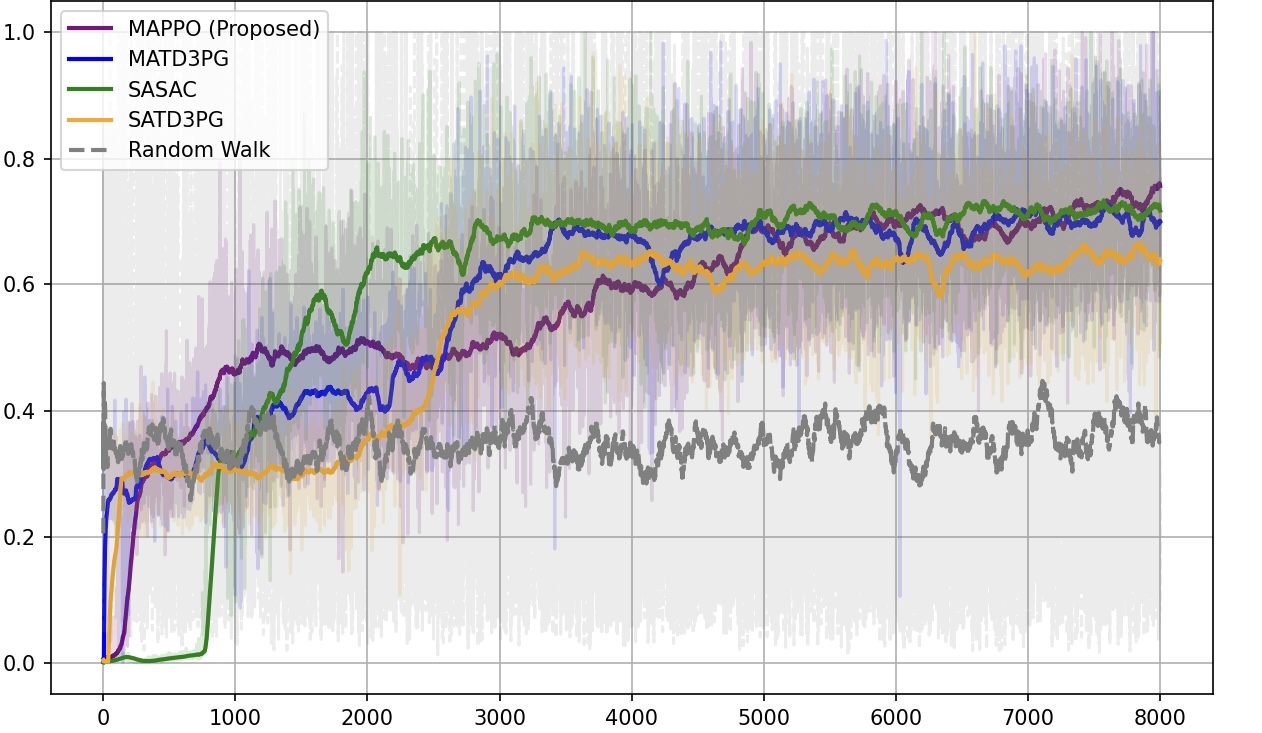
\includegraphics[width=\textwidth]{final.jpg}
    \caption{Convergence comparison showing the rolling 100-episode average multi-objective utility $U=\lambda_1\,\mathrm{ASSR}+\lambda_2\,P_d$ for all four RL algorithms (MAPPO, MATD3PG, SASAC, and SATD3PG) on the Week 9 system model.}
    \label{fig:rolling_secrecy}
\end{figure}

\section{Conclusion and Future Directions}
In this updated version of the 7 August report, we retain the original Week 9 semantic-aware ISAC system model while correcting the convergence-study objective to match the current implementation exactly. In particular, all five algorithms are now evaluated under the same episode-wise objective $\left(0.5\,\operatorname{ASSR} + 0.5\,P_d\right)\mathbb{I}_{\text{CRB}}$, where ASSR is normalized using a robust non-outlier secrecy reference and the CRB constraint is enforced through a Target-side feasibility indicator. The report also records the exact MAPPO hyperparameters used in the updated convergence script so that the optimization setup, implementation, and plotted results remain mathematically consistent and reproducible.

\bibliographystyle{IEEEtran}

\end{document}
